\documentclass[11pt]{article}
\usepackage{amsmath, amssymb, mathtools}
\usepackage{listings}
\usepackage{xcolor}
\usepackage{mdframed}
\usepackage{graphicx}
\usepackage[utf8]{inputenc} % per interpretare i caratteri UTF-8
\usepackage[T1]{fontenc}    % per una corretta codifica dei font
\usepackage{float}




\lstset{
  language=Matlab,         % Linguaggio MATLAB
  basicstyle=\ttfamily\footnotesize, % Tipo di carattere (monospazio) e dimensione
  numbers=left,           % Numeri di riga a sinistra
  numberstyle=\tiny\color{gray}, % Stile numeri di riga
  stepnumber=1,           % Un numero per ogni riga
  numbersep=8pt,          % Distanza tra numeri di riga e codice
  backgroundcolor=\color{black!5}, % Sfondo leggermente grigio chiaro
  showstringspaces=false, % Non visualizzare spazi tra le stringhe
  keywordstyle=\bfseries\color{cyan!70!black}, % Parole chiave in blu-verde
  commentstyle=\itshape\color{green!50!black}, % Commenti in verde italico
  stringstyle=\color{red!80!black}, % Stringhe in rosso
  identifierstyle=\color{purple}, % Identificatori (variabili) in viola
  breaklines=true,        % Linee lunghe si spezzano
  frame=single,           % Cornice attorno al codice
  framexleftmargin=5pt,   % Distanza tra il codice e la cornice a sinistra
  framexrightmargin=5pt,  % Distanza tra il codice e la cornice a destra
  framextopmargin=5pt,    % Distanza tra il codice e la cornice in alto
  %framebottommargin=5pt,  % Distanza tra il codice e la cornice in basso
  rulecolor=\color{black}, % Colore della cornice
  captionpos=b,           % Posizione della didascalia (opzionale)
  aboveskip=10pt,         % Distanza sopra il blocco di codice
  belowskip=10pt,         % Distanza sotto il blocco di codice
  lineskip=2pt,           % Distanza tra le righe
}

% Impostazione per visualizzare i risultati della console
\lstdefinestyle{console}{
  basicstyle=\ttfamily\footnotesize\color{black},
  backgroundcolor=\color{black!10}, % Leggero grigio per il fondo
  frame=single,          % Cornice attorno ai risultati
  rulecolor=\color{black}, % Colore della cornice
  captionpos=b,           % Posizione della didascalia
  aboveskip=10pt,         % Distanza sopra il blocco di codice
  belowskip=10pt,         % Distanza sotto il blocco di codice
  numbers=none,           % No numerazione delle righe
  showstringspaces=false, % Non mostra gli spazi nelle stringhe
  breaklines=true,        % Le linee troppo lunghe si spezzano
}






\begin{document}

\title{Metodi di Risoluzione degli Integrali}

\author{Tobia Sacchetto}
\date{\today}
\maketitle

%%%%%%%%%%%%%%%%%%%%%%%%%%%%%%%%%%%%%%%%%%
\section{Esercizio 1}
%%%%%%%%%%%%%%%%%%%%%%%%%%%%%%%%%%%%%%%%%%
\subsection{Consegna}
Preso dall'esercizio 8 della consegna. Calcolare una approssimazione del seguente integrale
\[
\int_0^\pi{\sin(x+1) dx}
\]
usando una formula di Gauss–Legendre a 4 punti. Fornire una stima dell’errore commesso in entrambe i casi (impostare il calcolo).

\[       
\begin{array}{ c c }
	x_i 	&	w_i		\\
	\hline
 -0.861136	&	0.347855 	\\
 -0.339981	&	0.652145 	\\  
  0.339981	&	0.652145  	\\
  0.861136	&	0.347855 	\\
\end{array}
\]
Fornire una stima dell’errore commesso (impostare il calcolo).
\subsection{Svolgimento}
Si ricorda che i $w_i$ sono i pesi per il polinomio di Legendre di grado 4, mentre gli $x_i$ sono le radici del polinomio sempre di $4^o$ grado di Legendre. 
Inoltre, il polinomio di Legendre vale solo per l'intervallo $[-1,1]$ quindi si richiede di trovare una formula per andare dall'intervallo $[0,\pi]$ a $[-1,1]$. \\
Si pone un ipotetico $t$ come incognita che se $x=0$ lo porti a $t=-1$ e se si pone $x=\pi$ lo porti a $t=1$:
\[
t=\frac{2x}{\pi}-1
\]
%-1 perché se inserisco 0 lo porto a -1,e poi di conseguenza mi concentro sui valori positivi. Se inserisco $\pi$ si annulla e diventa 2-1=1. Quindi questo vale anche per tutti i valori intermedi tra $\pi$ e 0.\\
A questo punto si isola l'incognita che diventa:
\[
x=\frac{\pi (t+1)}{2}\to dx=\frac{\pi}{2}dt
\]
 ora lo si sostituisce nell'integrale precedente:
\begin{align*}
	\int_0^\pi{\sin(x+1) dx} &= \int_{-1}^{1}{\sin(\underbrace{\frac{\pi}{2}(t+1)}_x+1)\frac{\pi}{2}dt}\\
	&=\frac{\pi}{2}\int_{-1}^{1}\underbrace{\sin(\frac{\pi}{2}(t+1)+1)dt}_{f}\\	
\end{align*}
Ora si può vedere l'integrale secondo il metodo di Gauss-Legendre come una sommatoria che va da 1 fino al grado del polinomio (4 in questo caso) e che all'interno moltiplica pesi per la funzione con le radici:
\[
\frac{\pi}{2}\int_{-1}^{1}f\\=\frac{\pi}{2}* \sum_{i=1}^4w_if(x_i)
\]
Si riporta di seguito un piccolo script MATLAB usato per i calcoli:
\begin{lstlisting}
close all
clear
clc

%%%%%%%%%%%%%%%%%
%               %
%% Esercizio 8 %%
%               %
%%%%%%%%%%%%%%%%%

f=@(x)(sin(pi/2 *(x+1)+1));
w=[0.347855 0.652145 0.652145 0.347855];
xi=[-0.861136 -0.339981 0.339981 0.861136];
risultato=0;
for i=1:4
    elemento=w(i)*f(xi(i));
    risultato=risultato+elemento;
end
risultato=pi/2 * risultato

errore=abs(2*cos(1)-risultato)


\end{lstlisting}
\subsection{Risultato}
Il risultato da console è:
\begin{lstlisting}[style=console]
risultato =

    1.0805962416823
    
errore =

   	8.3701e-06
\end{lstlisting}
Il risultato ottenuto svolgendo l'integrale è:
\[
\int_0^\pi{\sin(x+1) dx}=2\cos(1)=1.0806046117362794348018732
\]
Si noti che il risultato è approssimato bene fino alla quarta cifra dopo la virgola. Per l'esattezza l'errore è $8.3701e-06$, come calcolato con MATLAB
\subsection{Calcolo dell'errore}
Lo script precedente visualizzava anche l'errore che era stato commesso. Per impostare il calcolo dell'errore si prende la formula per il polinomio di grado 4 di Legendre:
\[
p_4(x)=\frac{1}{8}(35x^4-30x^2+3)
\]
e la si mette nella formula dell'errore, dove per $\xi$ si intende un valore per la $f$, $n=4=$ grado del polinomio, $a=-1$,$b=1$, $w(x)=1$ per le formule di Legendre e  $f=\sin(\pi/2 *(t+1)+1)$
\begin{align*}
	E[f]&=\frac{f^{(2n)}(\xi)}{(2n)!}\int_a^bw(x)p_n(x)^2dx\\
	&=\frac{f^{(8)}(\xi)}{(8)!}\int_{-1}^1w(x)p_4(x)^2dx\\
	&=\frac{f^{(8)}(\xi)}{(8)!}\int_{-1}^1({\frac{1}{8}(35x^4-30x^2+3)})^2dx\\
	&=\frac{\max_{x\in[-1,1]}(\frac{\pi^8\sin(\frac{\pi(x + 1)}{2} + 1)}{256})}{8!}\int_{-1}^1({\frac{1}{8}(35x^4-30x^2+3)})^2dx\\
	&=\frac{37.0645}{(8)!}*\frac{2}{9}\\
	&=2.0428e-04
\end{align*}
Di seguito viene visualizzata l'immagine della funzione $f^8$ per vedere visivamente il massimo. 
\begin{figure}[H]
  \centering
  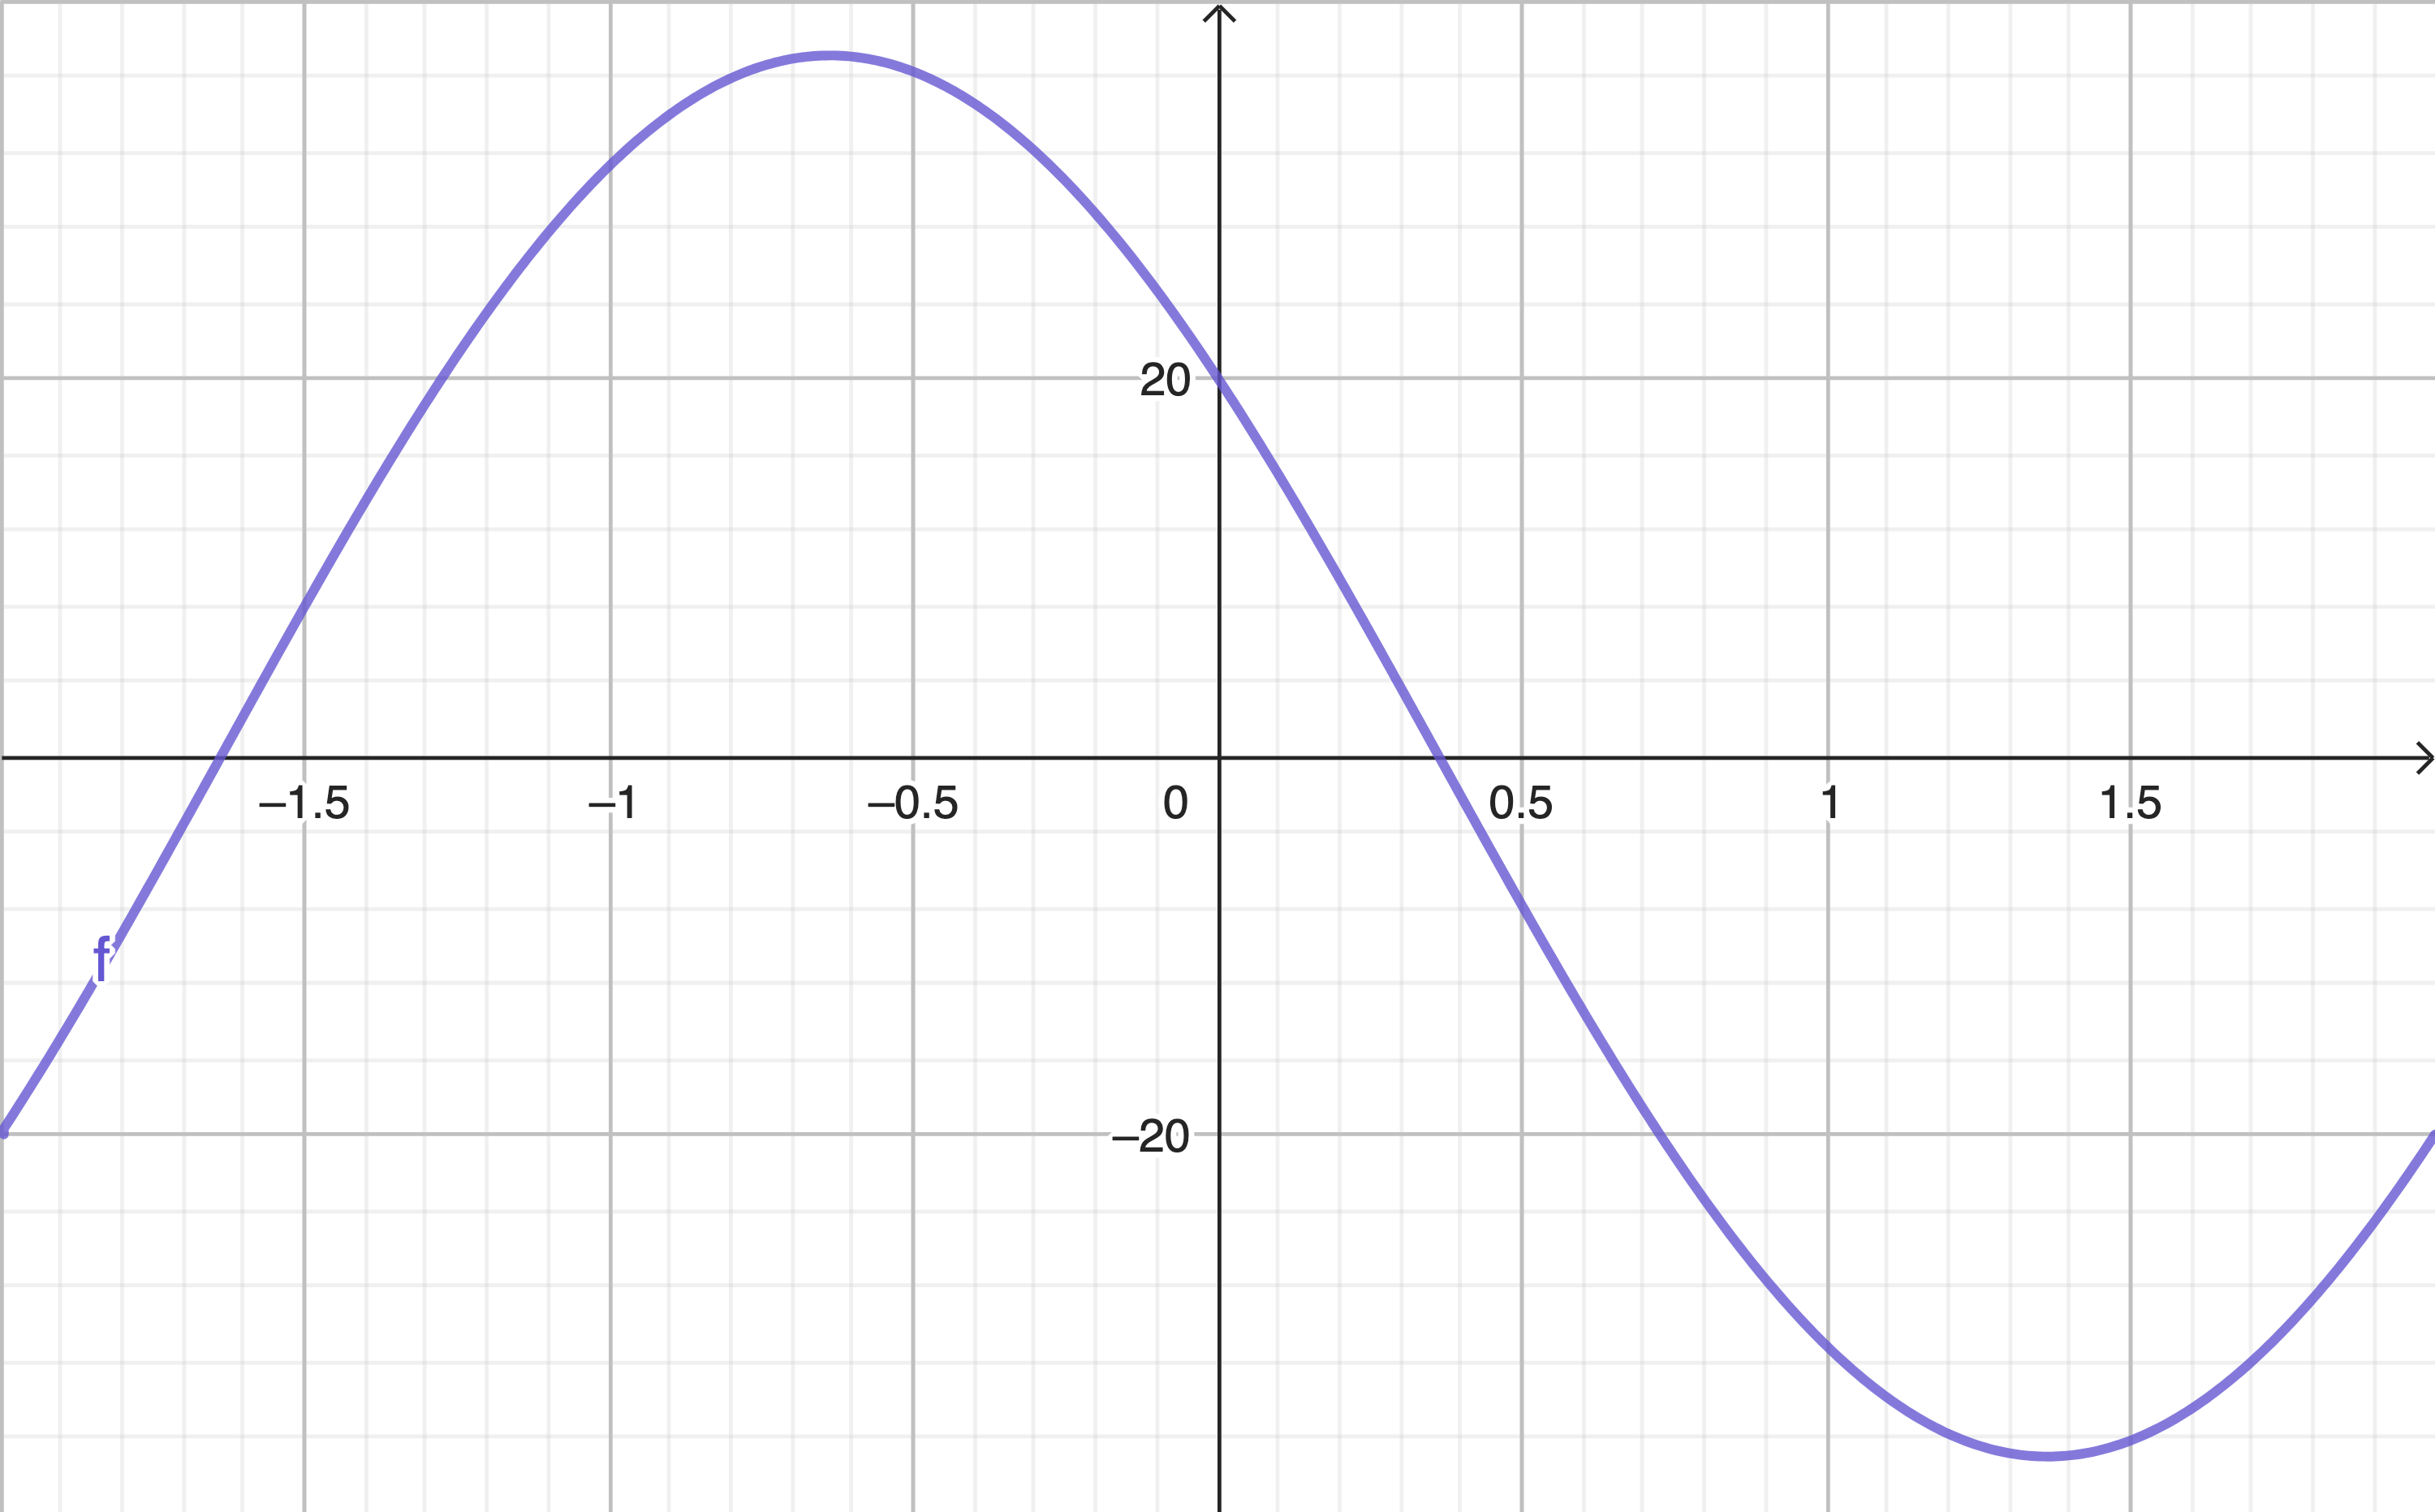
\includegraphics[width=0.7\textwidth]{images/errore.png} 
  \caption{Rappresentazione della funzione derivata $8^a$}
  \label{fig:funzione}
\end{figure}
Si osserva che l'errore calcolato precedentemente nella funzione è più piccolo ($8.3701e-06$) ed effettivamente lo maggiora.\\
Per fare i calcoli è stato usato MATLAB. Di seguito lo script, il quale calcola il massimo della funzione, l'integrale e successivamente l'errore
\begin{lstlisting}
close all
clear all
clc

%Calcolo derivata 8
% syms t
% f=sin(pi/2 *(t+1)+1);
% diff(f,8); 

%Trovo il massimo
z=@(x)((pi^8*sin((pi*(x + 1))/2 + 1))/256); %la mia derivata :)
[x_max, f_max_neg] = fminbnd(@(x) -z(x), -1, 1);
fprintf('Il massimo della funzione e: %d\n', z(x_max));
%Visualizzo la mia funzione
x_vals = linspace(-2, 2, 1000);
y_vals = z(x_vals); 
plot(x_vals,y_vals,'r');


%f=@(x)((1/8*(35*x^4-30*x^2+3))^2);
syms x
f=(1/8*(35*x^4-30*x^2+3))^2; %formula di legendre per il 4o grado
ris_int=int(f,x,-1,1); %risolvo l'integrale
errore=double(z(x_max)/factorial(8) * ris_int)
\end{lstlisting}
\section{Esercizio 2}
\subsection{Consegna}
Preso dall'esercizio 16: calcolare il seguente integrale
\[
\int_0^1{\int_0^x{\frac{y}{1+xy}dy}dx}
\]
usando regole di integrazione lungo la direzione x e y e tecniche di Montecarlo. Confrontare i risultati ottenuti in termini di accuratezza e complessità.
\subsection{Svolgimento}
Esistono vari possibili modi per svolgerlo con il metodo di Montecarlo. Si elencano 2 metodologie:
\subsubsection{Monte Carlo Crudo sul Dominio Triangolare}
Si generano i punti $(x,y)$ uniformemente distribuiti sul triangolo $0\leq y \leq x\leq1$. L'integrale è approssimato moltiplicando la media dei valori della funzione per l'area del triangolo (0.5). È riportato lo script MATLAB che risolve l'integrale usando il metodo descritto precedentemente.
\begin{lstlisting}
close all
clear 
clc

N=50000;                  %numero di punti
f=@(x,y)(y./(1+x.*y));    %funzione da integrare

x=rand(N,1); 
y=rand(N,1);

ind=find(y<=x);    %cerco le coppie (x,y) che stanno nel mio dominio
x=x(ind);               
y=y(ind);
I = 0.5*sum(f(x, y)) / length(ind); %moltiplico 0.5 per la media di f

fprintf('I=%g\n',I);
\end{lstlisting}
\subsubsection{Montecarlo Sequenziale}
Per ogni $x$ si stima l'integrale interno $\int_0^x{\frac{y}{1+xy}}dy$ con Monte Carlo. Successivamente, si valuta anche l'integrale esterno usando i valori ottenuti. È mostrato lo script MATLAB che risolve l'integrale usando il metodo appena descritto.
\begin{lstlisting}
close all
clear all
clc
N = 50000; % Campioni per l'integrale esterno
M = 50000; % Campioni per l'integrale interno
punti = rand(N, 1);
stima_integrale = 0;

for j = 1:N
    x_j = punti(j);
    y_i = x_j * rand(M, 1); % Campioni y ~ U(0, x_j)
    f_inner = y_i ./ (1 + x_j * y_i);
    I_xj = x_j * mean(f_inner); % Stima integrale interno
    stima_integrale = stima_integrale + I_xj;
end

stima_integrale = stima_integrale / N
\end{lstlisting}
\subsection{Differenze e Risultato}
Con entrambi i metodi si converge verso il valore $0.122$ con un numero sufficiente di campioni. Mentre il primo metodo è più efficiente e semplice, il secondo è utile per integrali annidati ma richiede più calcoli(aumenta la complessità).
\begin{itemize}
	\item Metodo 1: $0.122846151373576$ con $N=50000$
	\item Metodo 2: $0.122123789908462$ con $M=N=25000$
	\item Reale	: $0.122350853765048690185910429818425125976915434672702343633207713...$
\end{itemize}
I risultati (metodo 1 e 2) sono delle variabili aleatorie che cambiano casualmente di volta in volta che si lancia lo script, ma entrambe cercano di avvicinarsi al valore reale.
\section{Esercizio 3}
\subsection{Consegna}
Preso dall'esercizio 4:\\
Stimare quanti intervalli sono necessari nella formula composita dei trapezi per approssimare l’integrale
\[
\int^2_0\exp^{-x^2}dx
\]
con un’errore che sia minore di $10^{-6}$. Riprovare con il metodo di Romberg.
\subsection{Svolgimento}
\subsubsection{Trapezzi Composta}
La formula dei trapezzi composta è:
\[
\int_a^bf(x)dx=\frac{h}{2}(f(a)+2\sum_{i=0}^{h-1}f(x_i)+f(b))+E[f]
\]
dove, $h=\frac{b-a}{n}$, n=numero di valutazioni di funzioni, errore $=E[f]=-\frac{(b-a)h^2}{12}f''(\eta)$\\
Si pone $f=e^{-x^2}dx$, quindi $f''=4x^2e^{-x^2} - 2e^{-x^2}$.
Si crea la disequazione:
\[
|E[f]|\leq(b-a)^3\frac{M}{12n^2}=(b-a)\frac{h^2}{12}\max_{X\in[0,2]}|f''(x)| < 10^{-6}
\]
Si effettua la sostituzione e si procede con i calcoli:
\begin{align*}
	(2-0)\frac{{(\frac{2-0}{n})}^2}{12}\max_{x\in[0,2]}|4x^2e^{-x^2} - 2e^{-x^2}| &< 10^{-6}\\
	\frac{{(\frac{2}{n})}^2}{6}\max_{x\in[0,2]}|4x^2e^{-x^2} - 2e^{-x^2}| &< 10^{-6}\\
	\frac{2}{3n^2}\max_{x\in[0,2]}|4x^2e^{-x^2} - 2e^{-x^2}| &< 10^{-6}\\
	\frac{2}{3n^2}2 &< 10^{-6}\\
	\frac{4}{3n^2} &< 10^{-6}\\
	\frac{4}{3*10^{-6}} &< n^2\\
	1155\approx1154.7005\approx \sqrt{\frac{4}{3*10^{-6}}} &< n\\
\end{align*}
Lo script MATLAB utilizzato per il calcolo del massimo è riportato di seguito.Si visualizza graficamente la $f''$.
\begin{figure}[H]
  \centering
  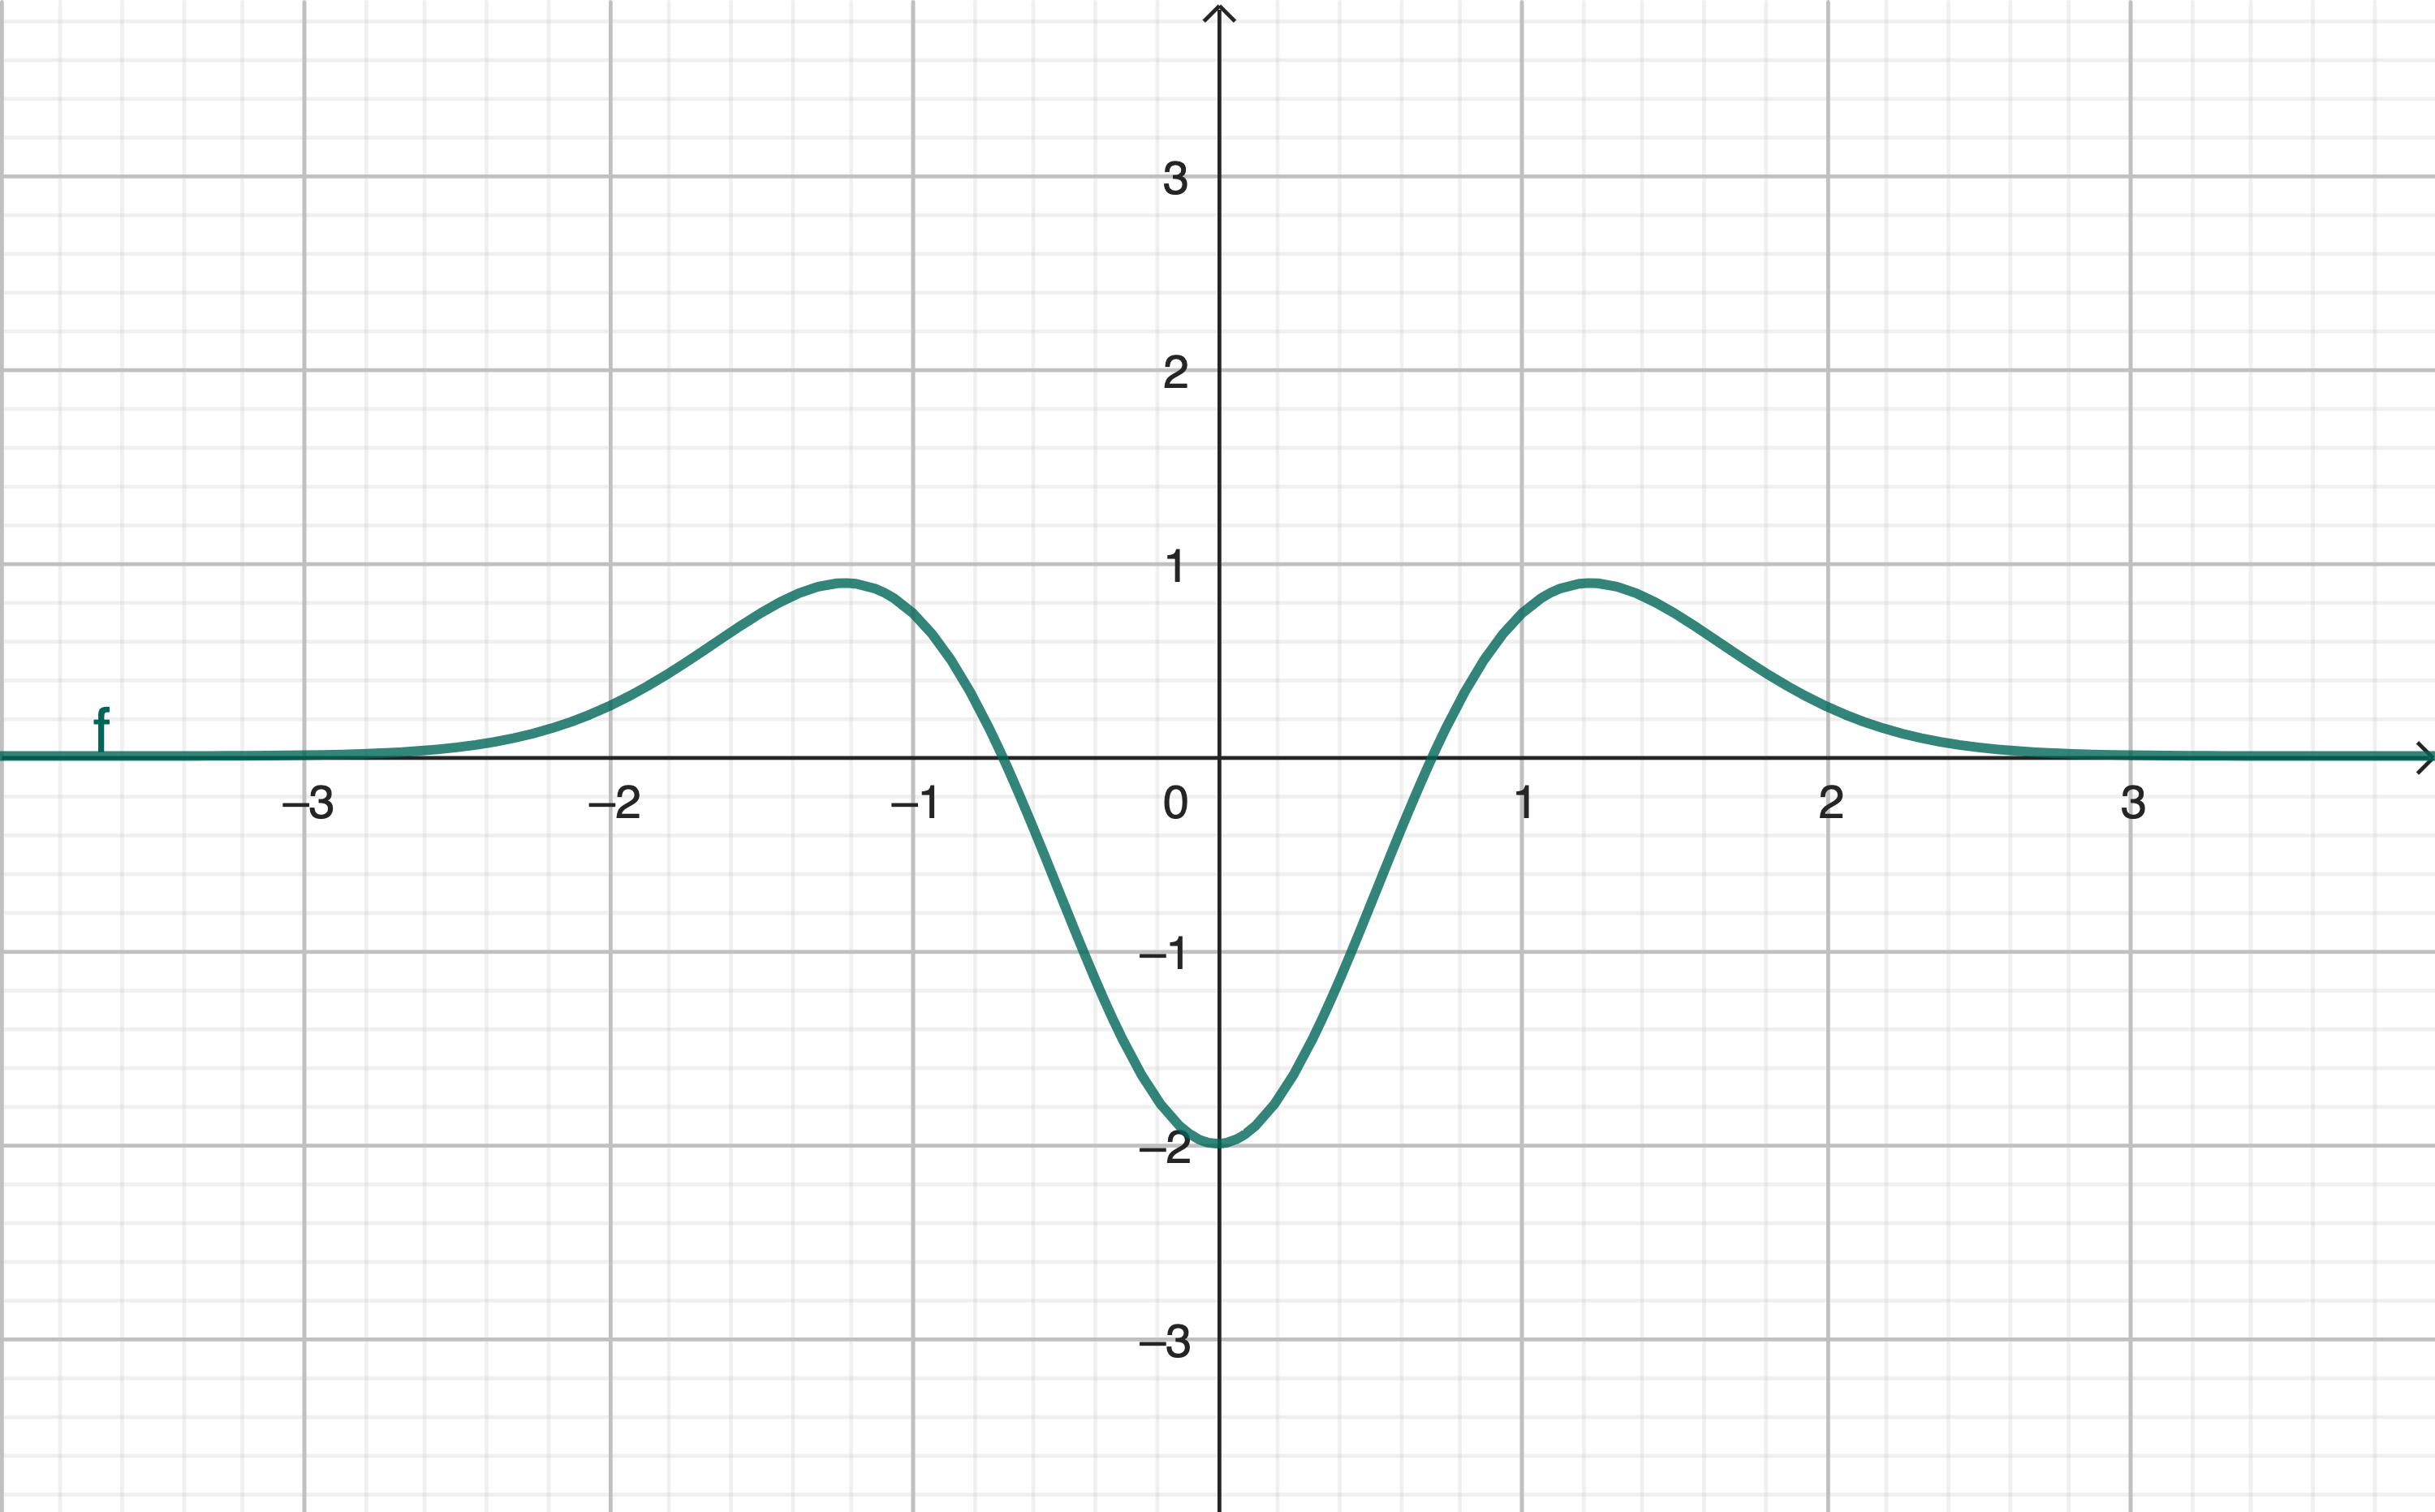
\includegraphics[width=0.7\textwidth]{images/funzione_max.png} 
  \caption{Rappresentazione della funzione}
  \label{fig:funzione}
\end{figure}
Come si può osservare il massimo è vicino a 2.
\subsubsection{Formula Romberg}
%Per trovare l'errore con Romberg si usa la seguente formula: $c(h)^{2n}$. Conosco $h$, metto h come $h=\left(\frac{b-a}{2^k}\right)^{2n}$. Non conosco $c$ e quindi devo calcolarmelo a forza di iterare. Quindi:
%\[
%h=2^{-k} \ \ \ \text{Errore}=O(h^{2k})\\
%\]
%\begin{table}[H]
%\centering
%\begin{tabular}{|c|c|c|}
%\hline
%\textbf{k} & \textbf{h} & \textbf{Errore} \\
%\hline
%1 & 0.5 	& 0.25 			\\
%2 & 0.25  	& 0.00390625  	\\
%3 & 0.125  	& 3.8147e-06 	\\
%4 & 0.0625  & 2.32831e-10 	\\
%\hline
%\end{tabular}
%\caption{Tabella per trovare $n$}
%\end{table}
%Mi sono fermato con $k=4$ perché il mio errore deve essere più piccolo di $e-06$. Abbiamo dunque trovato che ci servono $k=4$ iterazioni. Quindi $n=2^k=2^4=16$
%\begin{lstlisting}
%	
%\end{lstlisting}
Per trovare l'errore di Romberg ci si dota di un paio di formule. Si mostra la tabella dell'algoritmo di Romberg:
\[
\begin{array}{ c c c c c c }
	R_{1,1} 			\\
 R_{2,1}	&	R_{2,2} 	\\
 R_{3,1}	&	R_{3,2} & R_{3,3} 	\\  
  R_{4,1}	&	R_{4,2} & R_{4,3} & R_{4,4}  	\\
  R_{5,1}	&	R_{5,2} & R_{5,3} & R_{5,4} & R_{5,5} 	\\
  ... & ... & ... & ... & ... & ...\\
  \hline
  h_5^2 & h_5^4 & h_5^6 & h_5^8 & h_5^{10} & ... \\
 \end{array}
\]
Si ricordano un paio di informazioni. Il numero di iterazioni (k) è 5, ma nel trovare l'errore può anche non esserlo ed essere >5.  $R_{k,k}$ converge all’integrale come $h_k^{2k}$ dove $h$ è l'errore, $b=2$,$a=0$. Ora si pone:
\begin{align*}
h_k^{2k}&\leq 10^{-6} \\
\left(\frac{b-a}{2^{k-1}}\right)^{2k} &\leq 10^{-6}\\
\frac{2^{2k}}{2^{(k-1)2k}} &\leq 10^{-6}\\
2^{2k-(2k^2-2k)}&\leq 10^{-6}\\
2^{-2k^2+4k}&\leq 10^{-6}\\
\ln(2^{-2k^2+4k})&\leq\ln(10^{-6})\\
-2k^2+4k\ln(2)&\leq-6\ln(10)\\
-2k^2+4k&\leq -6\frac{\ln(10)}{\ln(2)}\\
-2k^2+4k+ 19.9316\geq0 \\
\end{align*}
Il risultato lo si può capire disegnando la funzione del polinomio nei punti in cui la funzione interseca l'asse delle x:
\begin{figure}[H]
  \centering
  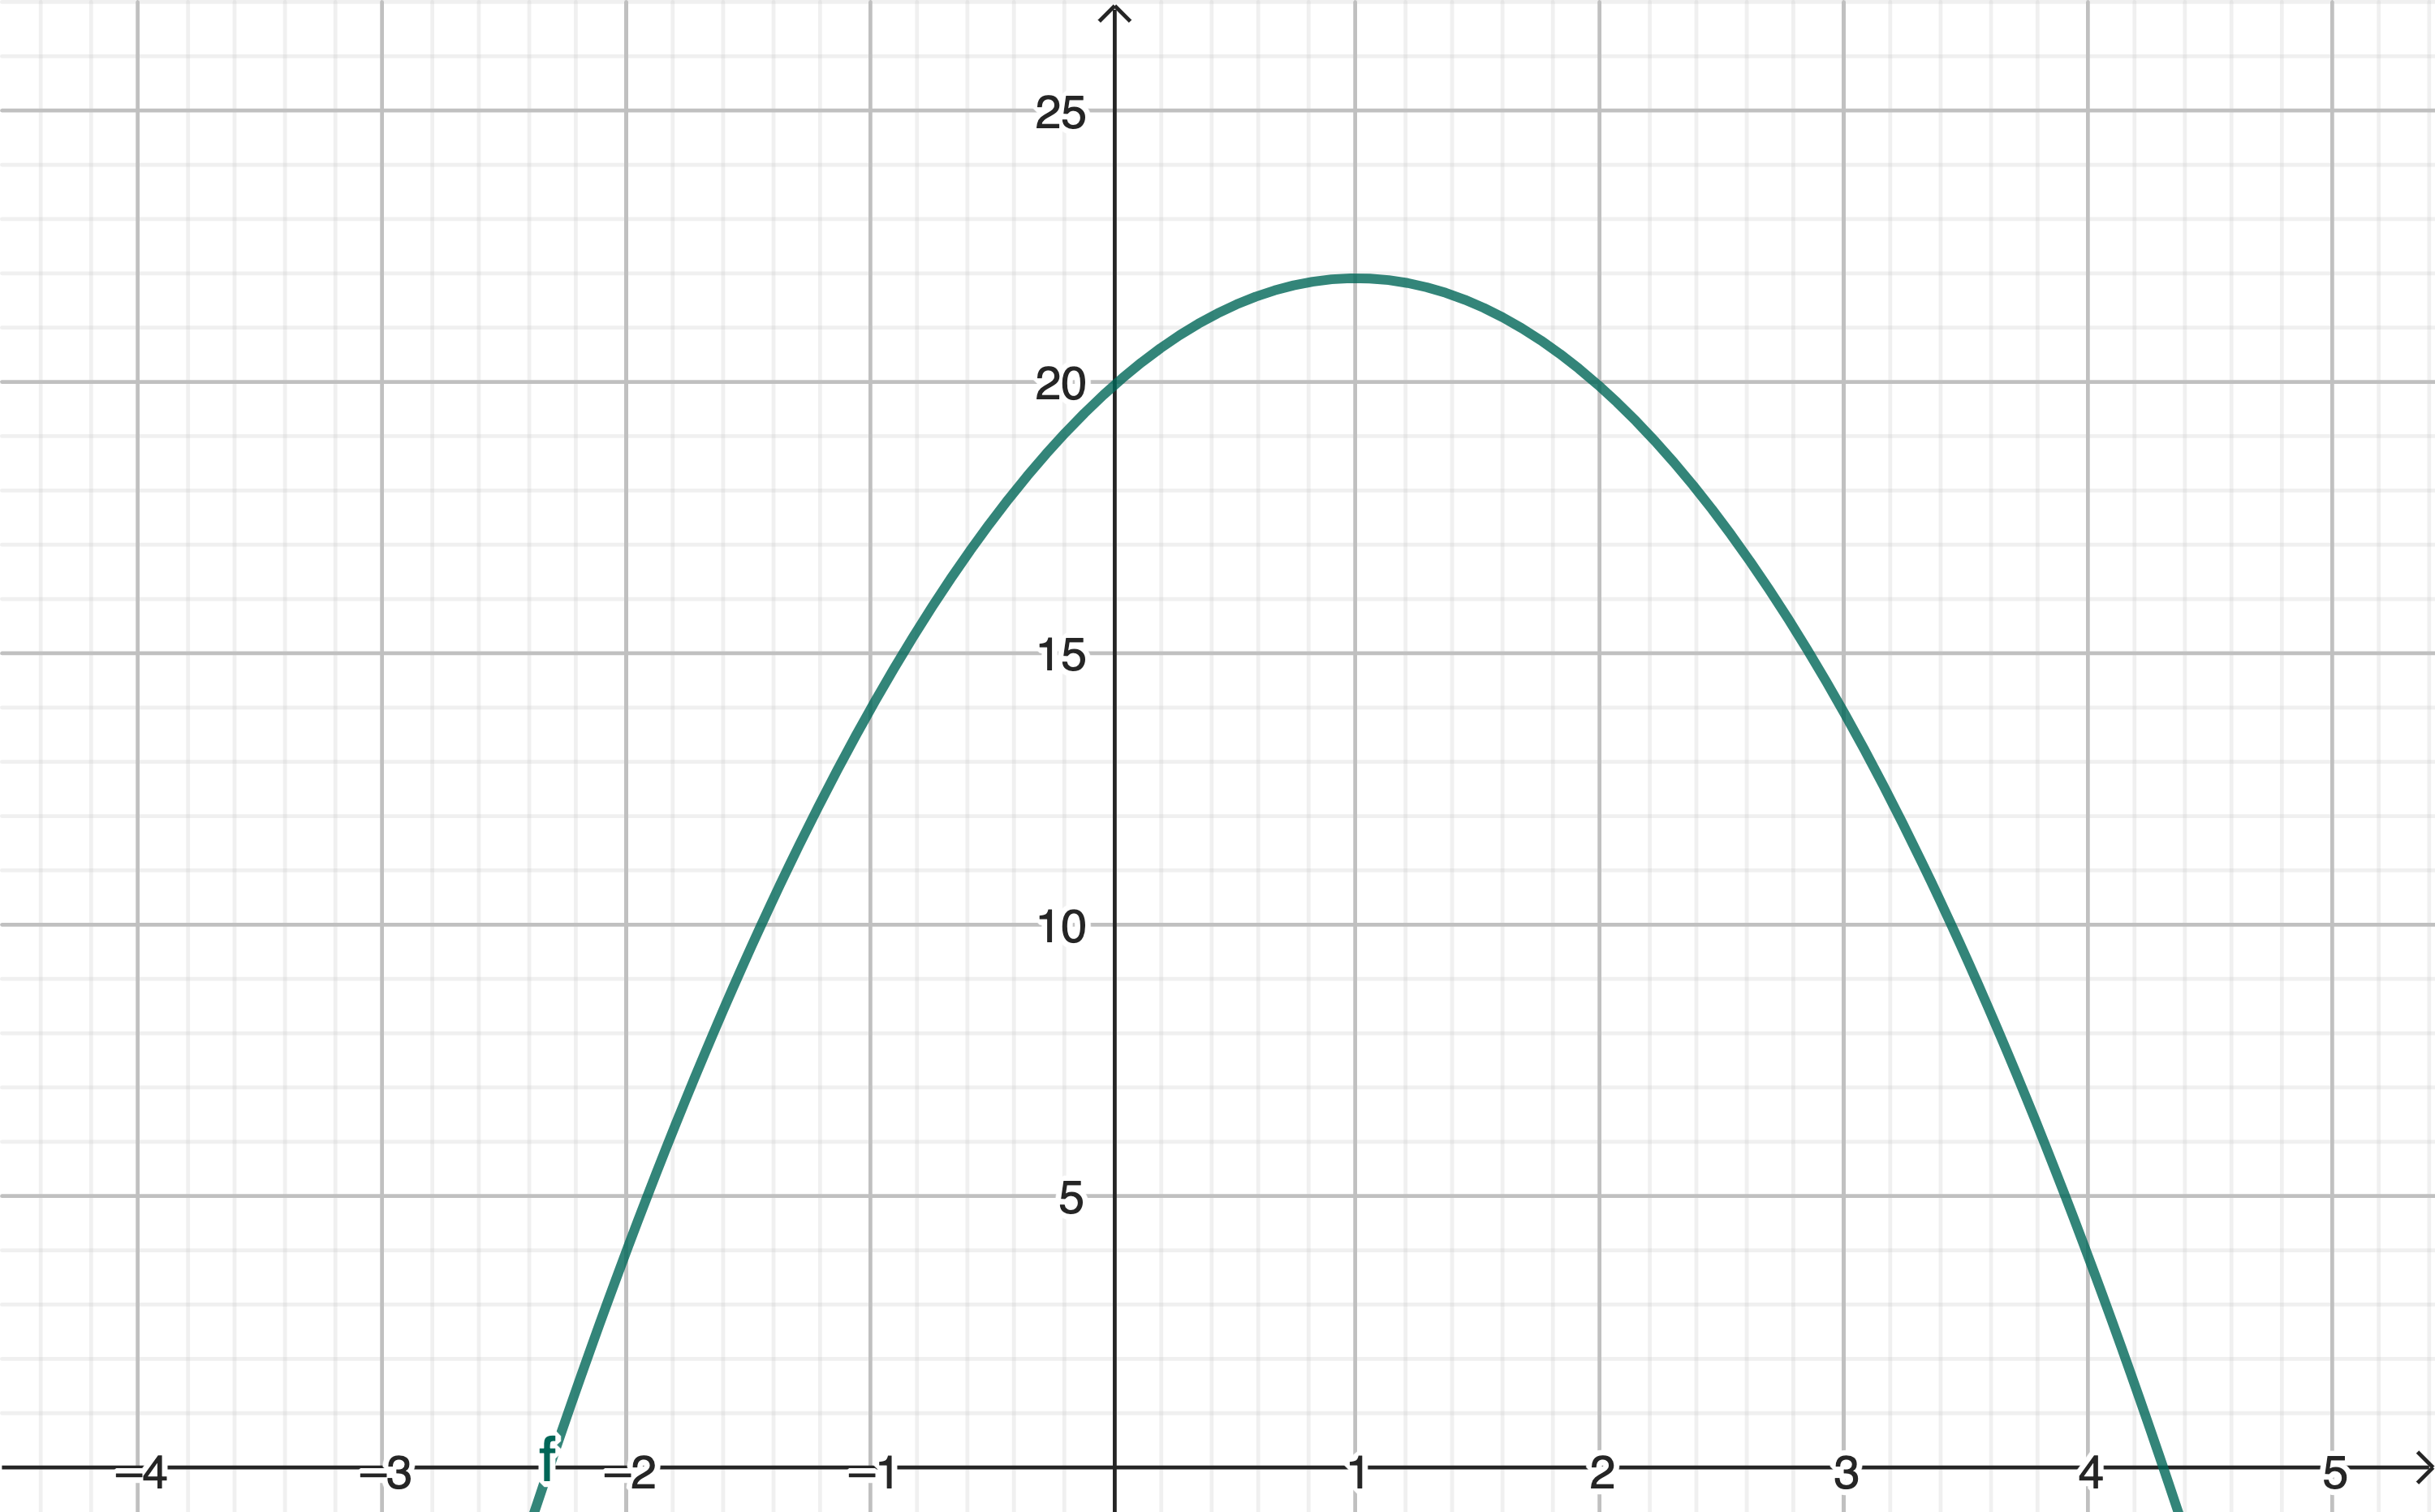
\includegraphics[width=0.7\textwidth]{images/polinomio.png} 
  \caption{Rappresentazione della funzione}
  \label{fig:funzione}
\end{figure}
Il risultato di conseguenza è $k_1=-2.311$ e $k_2=4.311$. Si prende il valore positivo e intero per eccesso dei risultati, quindi $k=5$.
La formula per trovare il numero di valutazioni di funzione è $2^{k-1} + 1$ che sostituendo diventa $2^{4} + 1=17$. Ora per scrupolo si esegue uno script in MATLAB per calcolare la tabella di Romberg e vedere se il numero $i$ (dove $R_{i,i}$ il valore più accurato sulla tabella) sia $\geq k$ e il numero di funzione sia $\geq$ del numero di funzioni che si è appena trovato.
\begin{lstlisting}
close all
clear
clc

%qua per trapezzi per trovare il massimo 
z=@(x)(abs(4*x^2*exp(-x^2) - 2*exp(-x^2)));
[x_max, f_max_neg] = fminbnd(@(x) -z(x), -1, 1);
fprintf('Il massimo della funzione f'' e: %d\n\n', z(x_max));



%Romberg
f=@(x)(exp(-x.^2));
tol=1e-6; %la nostra tolleranza
a=0;b=2;
m=inf;%numero di righe
%si ferma lui quando trova la tolleranza giusta


[R,k,itf,vett_val]=romberg(f,a,b,tol,m);
disp(R)
fprintf("\nIl valore e' stato trovato dopo %d iterazioni e quindi dopo %d valutazioni di funzione\n",k,size(vett_val,2));

\end{lstlisting}
\begin{lstlisting}
function [R,k,itf,vett_val]=romberg(f,a,b,tol,m)

h=b-a;
R(1,1)=h/2*feval(f,a)+feval(f,b);
vett_val=[a,b];
itf=2;
%M e' il numero delle righe
for k=2:m
    %La mia tabella e' costruita per righe
    R(k,1)=0.5*(R(k-1,1)+h*sum(feval(f,a+h/2:h:b-h/2))); %quello che faccio e' partire da a+h/2 e andare fino a b-h/2 con passo h 
    itf=itf+2^(k-2);
    vett_val=[vett_val, a+h/2:h:b-h/2];
    for i=2:k
        %adesso lavoro sulla riga i
        R(k,i)=(4^(i-1)*R(k,i-1)-R(k-1,i-1))/(4^(i-1)-1);
    end
    if(abs(R(k,k)-R(k-1,k-1))<=tol) %ho trovato la convergenza
        return
    end
    h=h/2; %aggiorno il passo
end
fprintf("Non ho trovato la convergenza\n");
\end{lstlisting}

\begin{lstlisting}[style=console]
Il massimo della funzione f' e: 2.389485e+00
	
1.0183         0         0         0         0         0
0.8770    0.8299         0         0         0         0
0.8806    0.8818    0.8853         0         0         0
0.8817    0.8821    0.8821    0.8820         0         0
0.8820    0.8821    0.8821    0.8821    0.8821         0
0.8821    0.8821    0.8821    0.8821    0.8821    0.8821


Il valore e' stato trovato dopo 6 iterazioni e quindi dopo 33 valutazioni di funzione
\end{lstlisting}
Come possiamo vedere $R_{i,i}=R_{6,6}$ e quindi $i=6>k=5$ e di conseguenza il numero di valutazione di funzione $33>17$.
\section{Esercizio 4}
\subsection{Consegna}
Preso dall'esercizio 3 del foglio.
Applicare il metodo di Romberg agli integrali dell’esercizio precedente (esercizio 2 del foglio) valutando quante valutazioni di funzioni occorrono per ottenere la stessa tolleranza $10^{-5}$
Per scrupolo si riportano gli integrali:
\begin{align*}
	\int^2_1\frac{1}{x}dx\\
	\int^1_{-1}\frac{1}{1+x^2}dx\\
	\int^2_0\cos(x)dx\\
\end{align*}
\subsection{Svolgimento}
\subsubsection{primo integrale}
Lo si svolge nel seguente modo:
\begin{align*}
	h_k^{2k}&= 10^{-5} \\
\left(\frac{b-a}{2^{k-1}}\right)^{2k} &=10^{-5}\\
\frac{1^{2k}}{2^{(k-1)2k}} &= 10^{-5}\\
(2^{1-k})^{2k}&=-5\ln(10)\\
2k(1-k)&= -5\frac{\ln(10)}{\ln(2)}\\
-2k^2+2k+ 16.61=0 \\
k_1&=3.43\\
k_2&=-2.43\\
\end{align*} 
Il valore che si mantiene è $k_1$ siccome positivo. Poichè la consegna chiede il numero di iterazioni esatto per avere una tolleranza di $10^{-5}$ allora lo si tiene così e non lo si approssima per eccesso ad un numero intero. Si calcola il numero di valutazioni di funzione: $2^{k-1}+1=2^{2.43}+1=6.3889$.
\subsubsection{secondo e terzo integrale}
Possiamo risolverli tutti e due con il seguente metodo:
\begin{align*}
	h_k^{2k}&= 10^{-5} \\
\left(\frac{b-a}{2^{k-1}}\right)^{2k} &=10^{-5}\\
\frac{2^{2k}}{2^{(k-1)2k}} &= 10^{-5}\\
-2k^2+4k&= -5\frac{\ln(10)}{\ln(2)}\\
2k^2-4k+ 16.61=0 \\
k_1&=-2.04\\
k_2&=4.04\\
\end{align*}
Si tiene solo $k_2$ perchè positivo. Valgono le stesse ipotesi descritte precedentemente col numero intero preso per eccesso. Si calcola il numero di valutazioni di funzione: $2^{k-1}+1=2^{3.04}+1=9.2821$.
\subsection{Prova dei Risultati ottenuti}
Adesso si prova a verificare se i risultati sono in linea con i valori ottenuti da MATLAB. Per trovare il numero di valutazione di funzioni si conosce la formula $2^{k-1}+1$. Si è fatto uso di un'apposita routine MATLAB, allegata al presente elaborato.
\subsubsection{MATLAB}
\begin{lstlisting}
close all
clear
clc

f=@(x)(1./x);
tol=1e-5;m=inf;
b=2;a=1;

f
[R,k,itf,vett_val]=romberg(f,a,b,tol,m);
disp(R);
fprintf("Numero di valutazioni di funzioni = %d, con k=%d iterazioni\n",size(vett_val,2),k);

f=@(x)(1./(1+x.^2));b=1;a=-1;
f
[R,k,itf,vett_val]=romberg(f,a,b,tol,m);
disp(R);
fprintf("Numero di valutazioni di funzioni = %d, con k=%d iterazioni\n",size(vett_val,2),k);

f=@(x)(cos(x));b=2;a=0;
f
[R,k,itf,vett_val]=romberg(f,a,b,tol,m);
disp(R);
fprintf("Numero di valutazioni di funzioni = %d, con k=%d iterazioni\n",2^(k-1)+1,k);
\end{lstlisting}
\begin{lstlisting}
function [R,k,itf,vett_val]=romberg(f,a,b,tol,m)

h=b-a;
R(1,1)=h/2*feval(f,a)+feval(f,b);
vett_val=[a,b];
itf=2;
%M e' il numero delle righe
for k=2:m
    %La mia tabella e' costruita per righe
    R(k,1)=0.5*(R(k-1,1)+h*sum(feval(f,a+h/2:h:b-h/2))); %quello che faccio e' partire da a+h/2 e andare fino a b-h/2 con passo h 
    itf=itf+2^(k-2);
    vett_val=[vett_val, a+h/2:h:b-h/2];
    for i=2:k
        %adesso lavoro sulla riga i
        R(k,i)=(4^(i-1)*R(k,i-1)-R(k-1,i-1))/(4^(i-1)-1);
    end
    if(abs(R(k,k)-R(k-1,k-1))<=tol) %ho trovato la convergenza
        return
    end
    h=h/2; %aggiorno il passo
end
fprintf("Non ho trovato la convergenza\n");
\end{lstlisting}
\subsubsection{Risultati}
I risultati sono rispettivamente:
\begin{itemize}
	\item Primo integrale con $15\geq 3.43$ iterazioni
e con $2^{15-1}+1=16385\geq 6.3889$ numero di valutazione di funzione 
	\item Secondo integrale con $6\geq 4.04$ iterazioni
e con $2^{6-1}+1=33\geq 9.2821.$ numero di valutazione di funzione 
	\item Terzo integrale con $5\geq 4.04$ iterazioni
e con $2^{5-1}+1=17\geq 9.2821.$ numero di valutazione di funzione 
\end{itemize}
Di conseguenza tutti i valora sopra riportati valgono.
\end{document}
